\section*{Q6}

The effects of k and s on speed are much more noticeable that for the simple decoder.
In Figure~\ref{swap}, we        

\begin{figure}
	\centering
	\begin{subfigure}{.8\linewidth}
		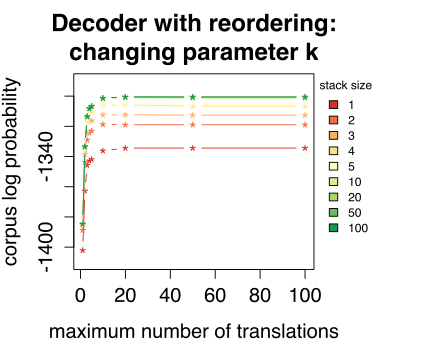
\includegraphics[scale=.75]{figures/d2_k.png}
		\caption{Increasing maximum number of translations, range [1--100].}
	\end{subfigure}
	\hskip2em
	\begin{subfigure}{.8\linewidth}
		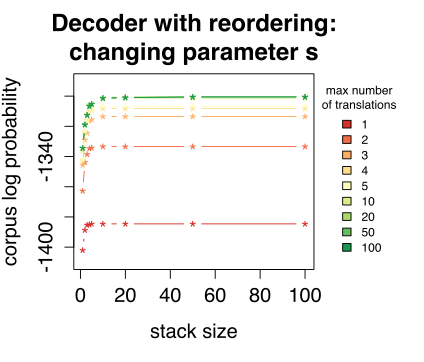
\includegraphics[scale=.75]{figures/d2_s.png}
		\caption{Increasing stack size, range [1--100].}
	\end{subfigure}
    \caption{Performance of decoder with local reordering.}\label{swap}
\end{figure}

\begin{figure}
	\centering
	\begin{subfigure}{.45\linewidth}
		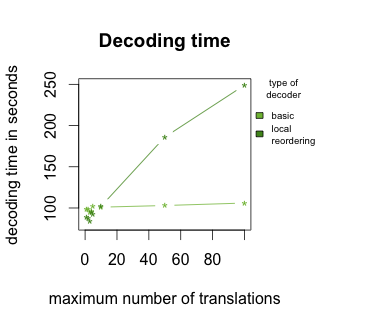
\includegraphics[scale=.55]{figures/k_time.png}
		\caption{Decoding time as function of maximum number of translations.}
	\end{subfigure}
	\hskip2em
	\begin{subfigure}{.45\linewidth}
		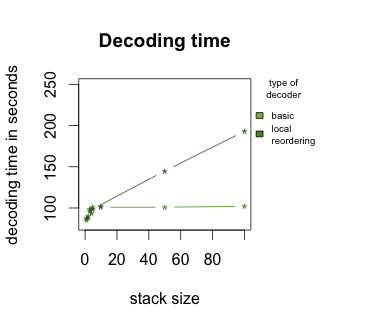
\includegraphics[scale=.55]{figures/s_time.png}
		\caption{Decoding time as a function of stack size.}
	\end{subfigure}
	\caption{Decoding time for the basic decoder and decoder with
    reordering.}\label{swaptime}
\end{figure}

